\chapter{Digital measurements}
\label{chap:extracting}
\textit{\textbf{Chapter abstract:} summary of the chapter, start to finish}
\section{Microcontrollers}
\label{sec:microcontrollers}
Microcontrollers are small programmable computers used to control input and output gates. These gates are commonly used to control digital and analog circuits. A microcontrollers quality is measured by the capacity of the chip (processor) and the size of the analog-to-digital converters (ADC). The speed or capacity of the chip is measured in Hertz (Hz) and is the speed of how many operations the microcontroller can complete per second. The ADC is a component that converts a analog signals from a circuit to a digital signal on one or more of the input gates. The conversion is done by the ADC in a microcontroller with sample-and-hold techniques to produce a digital signal from the varying input. The quality of an ADC is measured in how many bits the ADC consists of. This translates to how many steps in the analog to digital conversion it is capable of. This is also referred to as the resolution. For example, an 8 bit ADC will have a resolution of $2^{8} = 256$ (Figure \ref{fig:adc}). Small errors in the conversions are unavoidable, thus choosing a higher bit ADC will always be more beneficial. A few microcontrollers are considered for the task of producing digital signals from circuits as mentioned in Section \ref{chap:sensors}.

\begin{figure*}[!b]
    \centering
    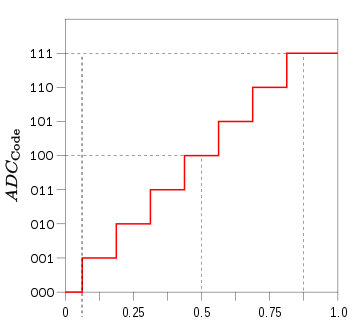
\includegraphics[width=0.49\textwidth]{figures/ADC_voltage_resolution.png}
    \caption{Concept of analog-to-digital conversion (Figure taken from \url{https://en.wikipedia.org/wiki/Analog-to-digital_converter})}
    \label{fig:adc}
\end{figure*}


\subsection{Raspberry Pi 3 Model A+}
1.4GHz Quad Core CPU, 512MB RAM, WiFi, BT, HDMI, MicroSD-card reader

\subsection{Arduino UNO Rev3}
\label{sec:arduinouno}
ATmega328P 16 MHz

\subsection{Arduino UNE}
Pros and cons, operating system, compatibility, ADC, sampling frequency, clock speed and ram.

\section{Software}
\label{sec:software}
This chapter gives and insight of which software was used

\subsection{Matlab}
\label{subsec:matlab}
What matlab is with pros and cons and how to generate plots.

\subsection{Arduino Software (IDE)}
The drivers used to read from the microcontroller

\section{Calibrating the system}
\label{sec:calibration}
The calibration of a pressure sensitive sensor can be done by calibrating the sensor at a minimum- and maximum-weight, adjusting the full-scale output. The output voltage is represented by forces loaded. This voltage can be calibrated and transformed directly to weight ($Kg$) for the specific sensor in use. Following, a line fit of the output full-scale can be created to make a system response of the system. This works well if we know the linearity of the measurements. If the conductance versus force linearity is known to increase more exponentially, we should consider using knots to section out certain parts of the full scale output.
\subsection{Calibration methods}
\label{subsec:calibrationmethods}
Calibration is an essential part of a measurement process and should be done regularly for consistent results. This section explains the concept of calibration why we do it.

\subsubsection{Modifying the full scale output}
The full scale output (FS) is the relation between input stimulus ($s$) and the output response. It defines the maximum value the system is able to output with given stimulus. Essentially, the full scale output is the measured voltage from the measurement system and can be modified digitally when reading the voltage.
The calibration method can typically be to create a system response based on a statistical line fitting model between a minimum- and maximum-value. For calibration in this thesis, we will see calibration be done with weights in five stages with different weights (also known as calibration knots). This is done by telling the system what weight has been loaded and referring this to the amount of voltage read by the micro controller (Chapter \ref{sec:microcontrollers}).

\subsection{Calibration weights}
For the sensors to be calibrated correctly, we are required to have a absolute scale of weights to refer our voltages to. This can be a certain amount of weights increasing linearly to the appropriate application area. For this thesis, a absolute scale can for example be from 1\si{\kilogram} to 20\si{\kilogram}.


\section{Chapter results}

\section{Chapter discussion}

\section{Summary}